\documentclass[aspectratio=169]{beamer}

% ----------------------------
% BASIC SETUP
% ----------------------------
\usepackage[utf8]{inputenc}
\usepackage[T1]{fontenc}
\usepackage{lmodern}     
\usepackage{amsmath, amssymb}
\usepackage{graphicx}
\usepackage{hyperref}
\usepackage{tikz}
\usepackage{pgfplots} 
\usepackage{placeins}

% ----------------------------
% REMOVE NAVIGATION SYMBOLS
% ----------------------------
\setbeamertemplate{navigation symbols}{}

% ----------------------------
% COLORS + SYLE
% ----------------------------
\definecolor{Accent}{RGB}{40,70,120} 
\setbeamercolor{title}{fg=Accent}
\setbeamercolor{frametitle}{fg=Accent}
\setbeamercolor{structure}{fg=Accent}
\newcommand{\kw}[1]{\textbf{\textcolor{Accent}{#1}}}
\setbeamertemplate{itemize item}{\raisebox{0.2ex}{\tiny$\blacktriangleright$}}
\setbeamertemplate{itemize subitem}{\raisebox{0.3ex}{\scriptsize$\bullet$}}
\setbeamertemplate{itemize subsubitem}{\tiny$\circ$}
% ----------------------------
% FONTS
% ----------------------------
\setbeamerfont{title}{series=\bfseries, size=\Large}
\setbeamerfont{frametitle}{series=\bfseries, size=\large}
\setbeamerfont{normal text}{size=\normalsize}

% ----------------------------
% FOOTLINE (minimal)
% ----------------------------
\setbeamertemplate{footline}{
    \hspace{1em}
    \scriptsize
    \textcolor{gray}{Ticketless Parking}
    %\hfill
    %\insertframenumber
    \hfill
    \textcolor{gray}{PS Distributed Systems}
    \hspace{1em}
}

% ----------------------------
% TITLE INFO
% ----------------------------
\title{Ticketless Parking}
\author{Dominik Schweigl, Nikola Adzic, Daniel Wenger}
\institute{Universität Innsbruck}
\date{}


% ----------------------------
% DOCUMENT
% ----------------------------
\begin{document}

% TITLE PAGE
\begin{frame}[plain]
    \vfill
    \titlepage
    \vfill
\end{frame}

% ----------------------------
\begin{frame}{System Architecture}
    \centering
    \includegraphics[width=0.9\linewidth, height=0.8\textheight, keepaspectratio]{architecture_diagram.png} 
\end{frame}

% ----------------------------
\begin{frame}{Resources (1/3)}
\begin{itemize}
    \item<+-> \kw{Dataset: Car License Plate Detection (Kaggle)}
    \begin{itemize}
        \item 400+ annotated images (front/rear views)
        \item Suitable for prototyping and evaluation
    \end{itemize}

    \item<+-> \kw{Computer Vision: YOLOv11 + OCR}
    \begin{itemize}
        \item Real-time license plate detection on the edge
        \item \textbf{OCR} extracts the license plate string
    \end{itemize}

    \item<+-> \kw{Messaging: NATS}
    \begin{itemize}
        \item Pub/Sub for camera frames and control signals (barrier)
        \item Asynchronous cloud-to-edge communication
    \end{itemize}
\end{itemize}
\end{frame}

% ----------------------------
\begin{frame}{Resources (2/3)}
\begin{itemize}
    \item<+-> \kw{Edge Stack: Python + SQLite + FastAPI + Akka}
    \begin{itemize}
        \item \textbf{Python} for ML integration
        \item \textbf{SQLite} as lightweight local store
        \item \textbf{FastAPI} to monitor barrier state and camera imput
    \end{itemize}

    \item<+-> \kw{Cloud Stack: Akka Typed + Akka HTTP + DynamoDB}
    \begin{itemize}
        \item Actor-based orchestration for \textit{parking lot} functionality
        \item \textbf{REST API} for edge and web clients
        \item Persistent actor state via \textbf{DynamoDB}
    \end{itemize}
\end{itemize}
\end{frame}

% ----------------------------
\begin{frame}{Resources (3/3)}
    \begin{itemize}
        \item<+-> \kw{Web Application: React + Tailwind CSS}
            \begin{itemize}
                \item \textbf{React} provides a dynamic UI for availability, reservations, routing and payments
                \item \textbf{Tailwind} CSS for responsive layout
                \item Browser-based \textbf{geolocation} supports finding nearby parking facilities
            \end{itemize}

        \item<+-> \kw{Hosting \& Deployment: EC2 + Nginx + Terraform (+ S3)}
        \begin{itemize}
            \item EC2 hosts the Akka backend and the web frontend on separate instances
            \item \textbf{Nginx} serves as webserver for the WebApp
            \item \textbf{Terraform} defines infrastructure as code; build artifacts are distributed via S3
        \end{itemize}
    \end{itemize}
\end{frame}
% ----------------------------


\begin{frame}{Live Demo}
\centering
\href{run:show3.mp4}{\texttt{Video}}
\end{frame}

% ----------------------------


\begin{frame}{Evaluation Result (1/3)}
\begin{columns}[T,totalwidth=\textwidth]

% LEFT: Summary
\begin{column}{0.35\textwidth}
\vspace{0.5em}
\kw{Cloud Backend (Load Test)}

\begin{itemize}
  \item Stable up to \kw{$\approx$300 req/s}
  \item Saturation at \kw{$\approx$400 req/s}
  \item Overload causes:
    \begin{itemize}
      \item high tail latency
      \item request timeouts
    \end{itemize}
\end{itemize}
\end{column}

% RIGHT: Plot
\begin{column}{0.65\textwidth}
\centering
\begin{tikzpicture}
\begin{axis}[
    width=\linewidth,
    height=0.7\textheight,
    xlabel={Target request rate [req/s]},
    ylabel={p95 latency [ms]},
    ymode=log,
    xmin=50, xmax=750,
    ymin=80, ymax=100000,
    grid=both,
    tick label style={font=\small},
    label style={font=\small},
]
\addplot+[black, mark=*, mark options={fill=black}, thick]
coordinates {
  (100,127)(200,126)(300,146)
  (400,3098)(450,6841)(480,17285)
  (500,30264)(520,37176)(540,62464)
  (560,60870)(580,66575)(600,52414)(700,63921)
};
\end{axis}
\end{tikzpicture}
\end{column}

\end{columns}
\end{frame}


% ----------------------------
\begin{frame}{Evaluation Result (1/3)}
\centering

\begin{tikzpicture}
\begin{axis}[
    width=0.9\linewidth,
    height=0.7\textheight,
    xlabel={Target request rate [req/s]},
    ylabel={Actual throughput [req/s]},
    xmin=50, xmax=750,
    ymin=0, ymax=500,
    grid=both,
    tick label style={font=\small},
    label style={font=\small},
]
\addplot+[black, mark=*, mark options={fill=black}, thick]
coordinates {
  (100,133)(200,233)(300,331)
  (400,418)(450,425)(480,298)
  (500,197)(520,128)(540,83)
  (560,70)(580,69)(600,76)(700,62)
};
\end{axis}
\end{tikzpicture}

\vspace{0.5em}

\end{frame}
% ----------------------------
\begin{frame}{Evaluation Result (1/3)}
\kw{Success Rate}
\\
\centering

\begin{tikzpicture}
\begin{axis}[
    width=0.9\linewidth,
    height=0.7\textheight,
    xlabel={Target request rate [req/s]},
    ylabel={Success rate [\%]},
    xmin=50, xmax=750,
    ymin=0, ymax=110,
    grid=both,
    tick label style={font=\small},
    label style={font=\small},
]
\addplot+[black, mark=*, mark options={fill=black}, thick]
coordinates {
  (100,100)(200,100)(300,100)
  (400,99.12)(450,79.56)(480,51.30)
  (500,50.25)(520,47.42)(540,45.95)
  (560,44.29)(580,41.89)(600,45.40)(700,42.18)
};
\end{axis}
\end{tikzpicture}

\vspace{0.5em}

\end{frame}

% ----------------------------

\begin{frame}{Evaluation Result (2/3)}
\kw{Web Interface Load Test} 
\\
\centering
\begin{tikzpicture}
\begin{axis}[
  width=0.95\linewidth,
  height=0.70\textheight,
  grid=both,
  xlabel={Target rate [req/s]},
  ylabel={Achieved rate [req/s]},
  ymin=0,
  legend style={at={(0.02,0.98)},anchor=north west,draw=none},
  tick label style={font=\small},
  label style={font=\small},
]
% Ideal tracking
\addplot[dashed] coordinates {
  (5,5) (10,10) (12,12) (14,14) (16,16)
  (18,18) (20,20) (22,22) (24,24)
  (26,26) (28,28) (30,30) (32,32) (34,34)
};
\addlegendentry{Ideal}

% Measured
\addplot[mark=*, thick] coordinates {
  (5,5.33) (10,9.76) (12,11.96) (14,13.86) (16,15.99)
  (18,11.52) (20,18.52) (22,19.88) (24,20.12)
  (26,22.95) (28,23.18) (30,25.88) (32,25.12) (34,13.29)
};
\addlegendentry{Measured}
\end{axis}
\end{tikzpicture}

\vspace{0.2em}

\end{frame}
% ----------------------------
\begin{frame}{Evaluation Result (2/3)}
\kw{Nginx Server Response Latency}
\\
\centering
\begin{figure}[H]
\centering
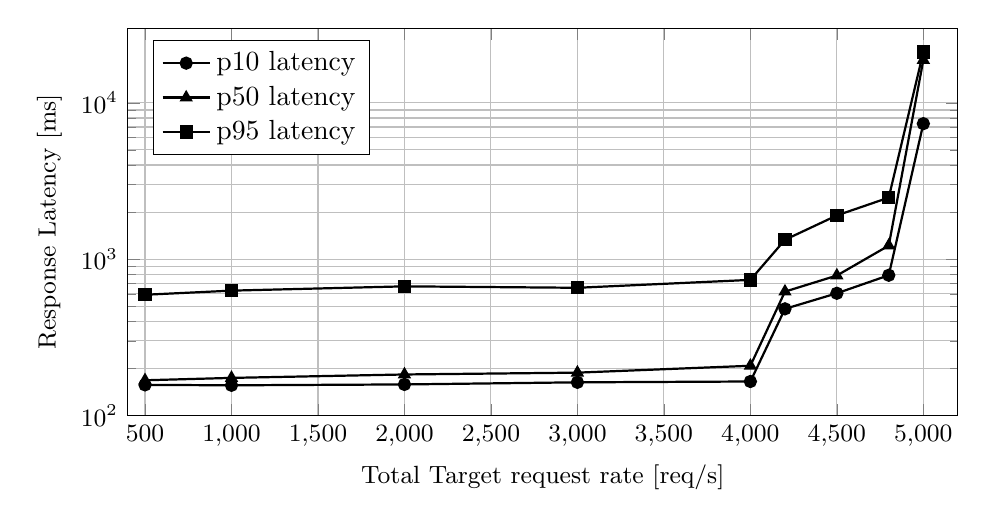
\begin{tikzpicture}
\begin{axis}[
    width=\linewidth,
    height=6.5cm,
    xlabel={Total Target request rate [req/s]},
    ylabel={Response Latency [ms]},
    ymode=log,
    xmin=400, xmax=5200,
    ymin=100, ymax=30000,
    grid=both,
    legend style={at={(0.03,0.97)},anchor=north west},
    tick label style={font=\small},
    label style={font=\small},
]

% p10
\addplot+[black, mark=*, thick, mark options={
    fill=black,
    draw=black 
  }]
coordinates {
  (500,157)
  (1000,156)
  (2000,158)
  (3000,163)
  (4000,165)
  (4200,481)
  (4500,605)
  (4800,789)
  (5000,7355)
};
\addlegendentry{p10 latency}

% p50
\addplot+[black, mark=triangle*, thick, mark options={
    fill=black,
    draw=black 
  }]
coordinates {
  (500,168)
  (1000,174)
  (2000,183)
  (3000,188)
  (4000,208)
  (4200,620)
  (4500,786)
  (4800,1221)
  (5000,18814)
};
\addlegendentry{p50 latency}

% p95
\addplot+[black, mark=square*, thick, mark options={
    fill=black,
    draw=black 
  }]
coordinates {
  (500,592)
  (1000,629)
  (2000,670)
  (3000,656)
  (4000,737)
  (4200,1330)
  (4500,1904)
  (4800,2476)
  (5000,21145)
};
\addlegendentry{p95 latency}

\end{axis}
\end{tikzpicture}
\label{fig:nginx-latency}
\end{figure}



\end{frame}
% ----------------------------
\begin{frame}{Evaluation Result (2/3)}
\kw{Nginx Throughput}
\\
\centering
\begin{figure}[H]
\centering
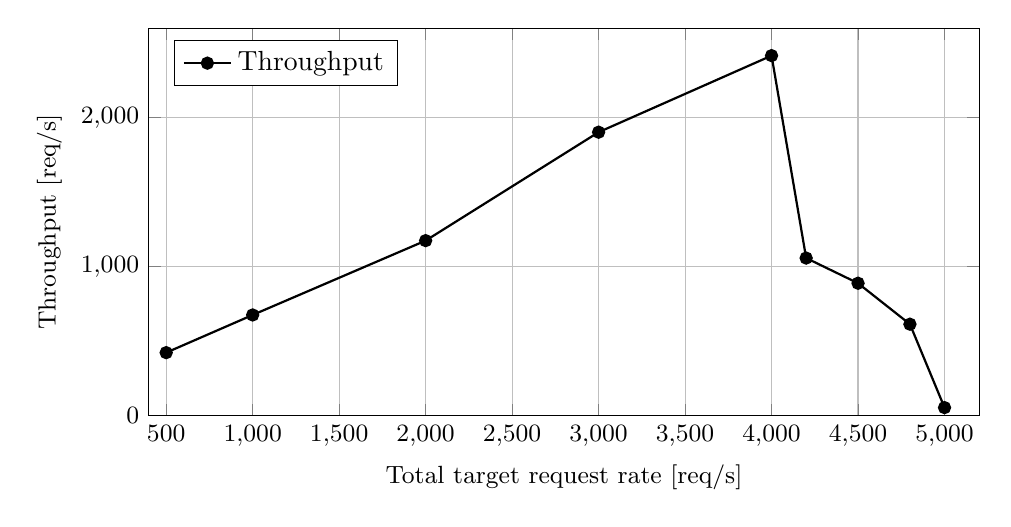
\begin{tikzpicture}
\begin{axis}[
    width=\linewidth,
    height=6.5cm,
    xlabel={Total target request rate [req/s]},
    ylabel={Throughput [req/s]},
    xmin=400, xmax=5200,
    ymin=0, ymax=2600,
    grid=both,
    legend style={at={(0.03,0.97)},anchor=north west},
    tick label style={font=\small},
    label style={font=\small},
]

\addplot+[black, mark=*, mark options={fill=black}, thick]
coordinates {
  (500,422)
  (1000,675)
  (2000,1174)
  (3000,1902)
  (4000,2416)
  (4200,1057)
  (4500,888)
  (4800,613)
  (5000,53)
};
\addlegendentry{Throughput}

\end{axis}
\end{tikzpicture}
\end{figure}
\end{frame}
% ----------------------------
\begin{frame}{Evaluation Result (3/3)}
\kw{Latency Distribution (Entry)}
\\
\begin{figure}[t]
\centering
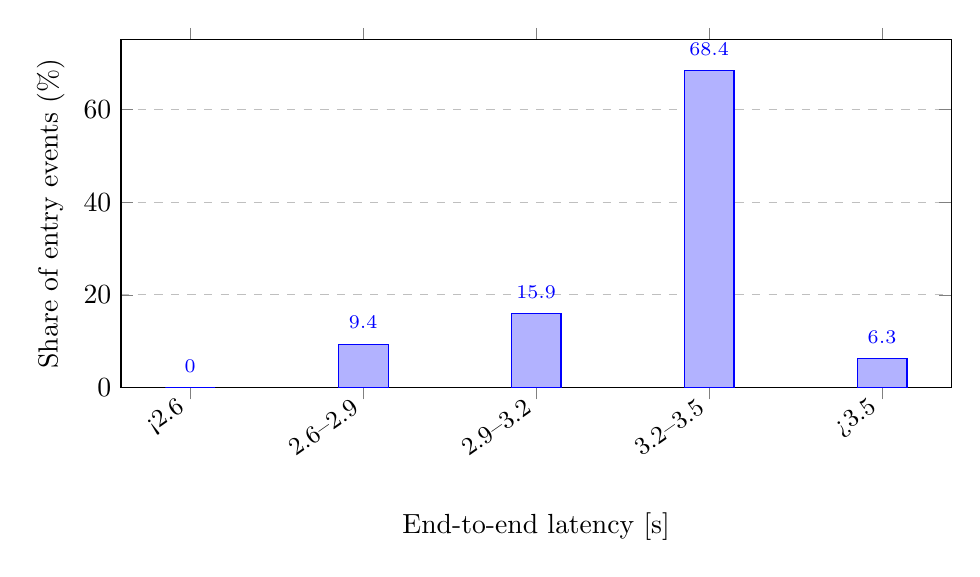
\begin{tikzpicture}
\begin{axis}[
  ybar,
  bar width=18pt,
  ymin=0,
  ymax=75,
  ylabel={Share of entry events (\%)},
  xlabel={End-to-end latency [s]},
    xlabel style={
    yshift=-12pt
  },
  symbolic x coords={<2.6,2.6--2.9,2.9--3.2,3.2--3.5,>3.5},
  xtick=data,
  xticklabel style={
    rotate=35,
    anchor=east,
    font=\small
  },
  nodes near coords,
  nodes near coords align={vertical},
  every node near coord/.append style={
    font=\scriptsize,
    yshift=2pt
  },
  ymajorgrids,
  grid style={dashed},
  width=\linewidth,
  height=6cm,
]

\addplot coordinates {
  (<2.6, 0.0)
  (2.6--2.9, 9.4)
  (2.9--3.2, 15.9)
  (3.2--3.5, 68.4)
  (>3.5, 6.3)
};

\end{axis}
\end{tikzpicture}
\end{figure}
\vspace{0.3em}
\scriptsize Total exit samples: 414
\end{frame}
% ----------------------------
\begin{frame}{Evaluation Result (3/3)}
\kw{Latency Distribution (Exit)}
\centering
\begin{figure}[t]
\centering
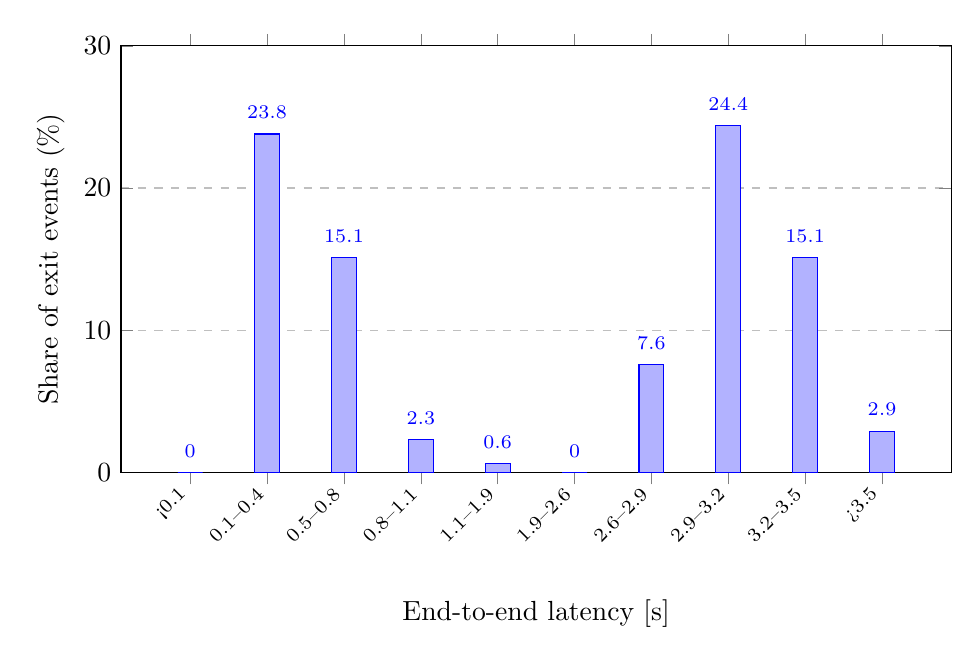
\begin{tikzpicture}
\begin{axis}[
  ybar,
  bar width=9pt,
  ymin=0,
  ymax=30,
  ylabel={Share of exit events (\%)},
  xlabel={End-to-end latency [s]},
  xlabel style={
  yshift=-12pt
  },
  symbolic x coords={
    <0.1,
    0.1--0.4,
    0.5--0.8,
    0.8--1.1,
    1.1--1.9,
    1.9--2.6,
    2.6--2.9,
    2.9--3.2,
    3.2--3.5,
    >3.5
  },
  xtick=data,
  xticklabel style={
    rotate=45,
    anchor=east,
    font=\scriptsize
  },
  nodes near coords,
  nodes near coords align={vertical},
  every node near coord/.append style={
    font=\scriptsize,
    yshift=2pt
  },
  ymajorgrids,
  grid style={dashed},
  width=\linewidth,
  height=7cm,
]

\addplot coordinates {
  (<0.1, 0.0)
  (0.1--0.4, 23.8)
  (0.5--0.8, 15.1)
  (0.8--1.1, 2.3)
  (1.1--1.9, 0.6)
  (1.9--2.6, 0.0)
  (2.6--2.9, 7.6)
  (2.9--3.2, 24.4)
  (3.2--3.5, 15.1)
  (>3.5, 2.9)
};

\end{axis}
\end{tikzpicture}

\end{figure}

\vspace{0.3em}
\scriptsize Total exit samples: 172
\end{frame}


% ----------------------------

\begin{frame}{Thank you for your attention!}
    \centering
    Questions?
\end{frame}


\end{document}